% !TeX root = Bericht.tex
% !TeX spellcheck = en_US
\section{Theory}
\label{sec:theorie}

In this section, the basic theoretical principles are briefly outlined to provide a better understanding of what a Gaussian beam is and how a cavity works.

\subsection{Gaussian beam}
The Gaussian modes are a set of solutions to the Helmholtz equation, which can be derived from Maxwell's equations using the paraxial approximation (see \autocite{gaussian_beam_script}). Their intensity is given by 
$$ I(x,y,z) \sim |U(x,y,z)|^2=I_0\left(\frac{w_0}{w(z)}\right)^2 \cdot \exp\left(-2\frac{x^2+y^2}{w(z)^2}\right)$$
, where $w_0$ is the beam radius when in focus (also known as the beam waist), $w(z)$ is the radius of the beam at a given location $z$, $I_0$ is the original intensity of the laser and $y$ is the spacial expansion. The beam width is given by
\begin{equation}\label{eqn:wz}
	w(z)=w_0\sqrt{1+\left(\frac{z}{z_R}\right)^2}\ .
\end{equation}
Here $z_R = \pi\cdot w_0/\lambda$ is called the Rayleigh length, which is given by the distance at which the intensity decreases by the factor $1/e^2$, at this point the beam width increases by $\sqrt{2}$. Via geometrical analysis, expressions for the curvature of the beam $R(z)$ and the divergence angle $\theta$ can be found (see \autocite{gaussian_beam_script}).

The Rayleigh length divides the beam into two regimes, a near field, where the beam can be regarded as a plane wave (curvature $R=\infty$) and far field, where the beam can be regarded as a cubic wave ($R(z)\sim z$). 

\subsection{Matrix formalism}\label{subsec:matrix}
In order to describe the effect of optical elements on a Gaussian beam, the ABCD matrix formalism can be used. Therefore, we define a complex quantity $q(z)$, such that
$$\frac{1}{q(z)} = \frac{1}{R(z)}- i\frac{\lambda}{\pi w(z)^2}.$$
When passing an optical element, the complex quantity changes according to
$$\frac{1}{q_2}=\frac{C+D/q_1}{A+B/q_1}.$$
The parameters $A,B,C,D$ are entries of a $2 \times 2$ matrix. The form of the matrices for free propagation, lenses and mirrors are given in \autoref{fig:matrix_optics_table}. Combination of optical elements is done via matrix multiplication, where the multiplication order corresponds to the order of propagation.

\begin{figure}[H]
	\centering
	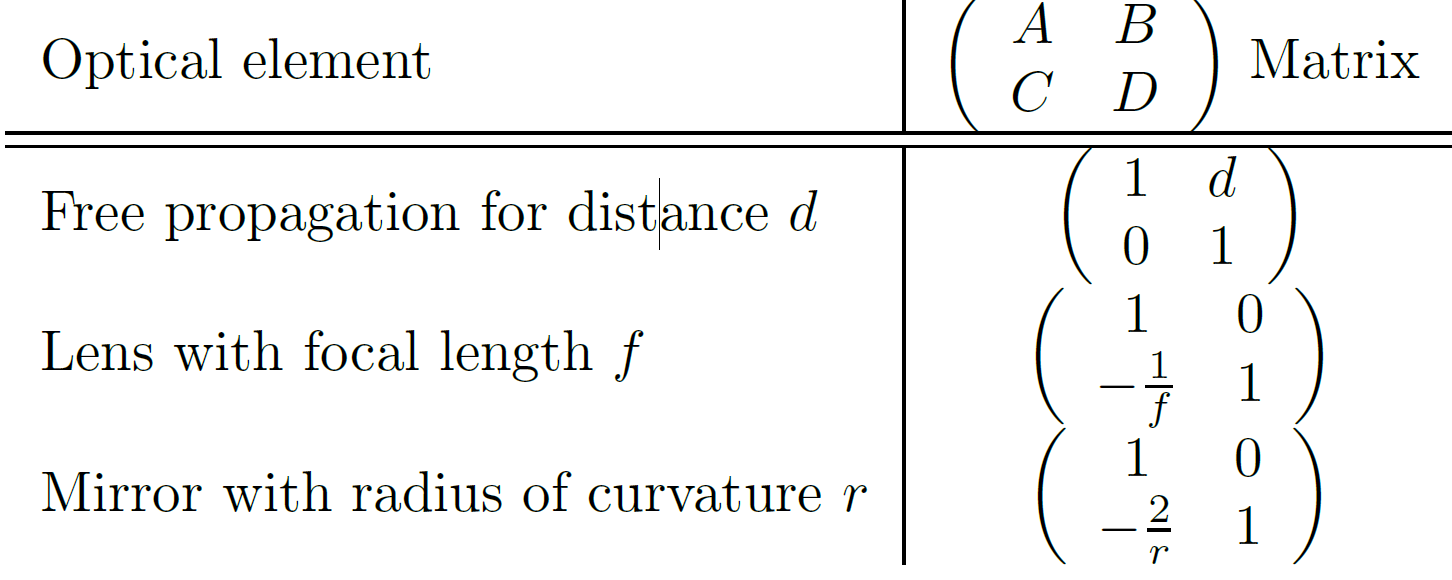
\includegraphics[width=0.55 \textwidth]{Bild_2024-04-11_005434519}
	\caption{Matrix entries for lenses, mirrors and free propagation in space. Table taken from \autocite{gaussian_beam_script}.}
	\label{fig:matrix_optics_table}
\end{figure}

Using this formalism, we can calculate the beam waist $w_2$ of an incident collimated beam with waist $w_1$ and curvature $R = \infty$ at a distance $z = f$ after passing through a lens with focal length $f$. The result

\begin{equation}\label{eqn:w2}
	 w_2 = \sqrt{\frac{f^2w_1^2\lambda^2}{\pi^2w_1^4 + f^2\lambda^2}} \approx \frac{f\lambda}{\pi w_1}
\end{equation}
can be further simplified, assuming $f^2\lambda^2$ to be negligibly small.

\subsection{Optical Resonator}
\label{subsec:OptRes}
In an optical resonator, two mirrors are set up parallel to each other at a certain distance $L$. Due to the fact that the electric field has a node at each mirror, only waves with a wavelength $\lambda$ that is an integer inverse of the half distance between those mirrors can exist as standing waves. So we get the general relation
$$\lambda_n=\frac{2 L}{n}, $$ 
where $n$ is an integer. Changing wavelength to frequency $\nu$ and introducing the free spectral range (FSR) as $\Delta \nu_{\mathrm{FSR}}= c/2L$ the relation can be simplified to $\nu=n\Delta \nu_{\mathrm{FSR}}$ (see~\autocite{diodenlaser}).
If the mirrors are semi-transparent, monochromatic light can be transmitted. Depending on the reflectivity, other frequencies can also pass through the mirror and the peaks smooth out \autocite{Fabry-Perot_Interferometer_Tutorial}. 
%This behavior is shown in \autoref{fig:Reflexivität}. 

%\begin{figure}[H]
%	\centering
%	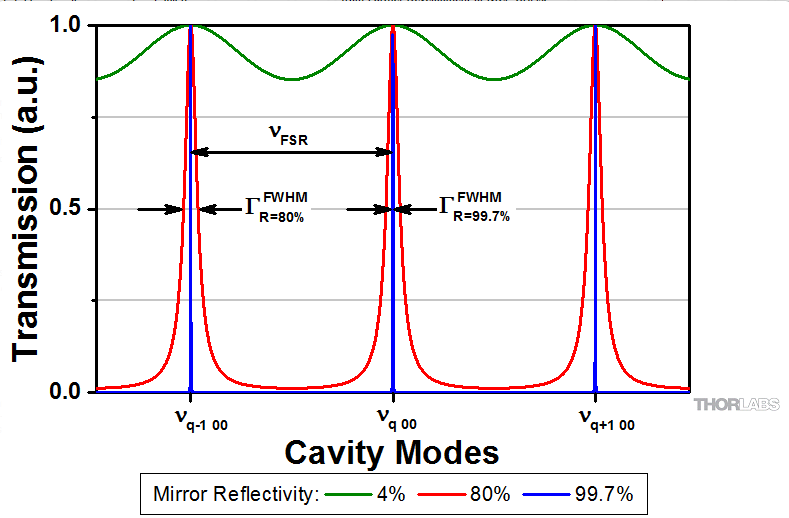
\includegraphics[clip,trim=0 0 0 2, width=0.9\linewidth]{Bild Reflektivität}
%	\caption{\glqq Mode spectrum of a Fabry-Pérot interferometer for mirror reflectances of 99.7\%, 80\%, and 4\%, illustrated by a blue, red, and green curve, respectively. 99.7\% reflectance corresponds to the case for the SA200 series, which has a free spectral range of 1.5 GHz. The 4\% reflectance corresponds to a typical "fringing effect" arising from reflections between parallel surfaces on glass plates.\grqq 
%		From \autocite{Fabry-Perot_Interferometer_Tutorial}.}
%	\label{fig:Reflexivität}
%\end{figure}

To quantify the quality of a cavity, we introduce the finesse $\mathcal{F}$ of a cavity, defined as the ratio between the FSR and full width at half minimum (FWHM) of the transmitted peaks. Assuming all losses coming from mirror transmission, we can theoretically compute the finesse. Both relations are listed below
\begin{equation}\label{eqn:finesse}
	\mathcal{F}_{\text{exp}} = \frac{\Delta \nu_{\mathrm{FSR}}}{\text{FWHM}} \qquad \mathcal{F}_{\text{theo}} = \frac{\pi\sqrt{R}}{1 - R},
\end{equation}
with $R$ being the mirror reflectivity.

A confocal resonator has a special geometry, where both mirrors are curved with the same radius $r$ as the length $L$ between them ($r = L$). This has some essential benefits, such as the fact that when correctly aligned the stability is very high. Additionally, if the laser beam is misaligned, we only get one peak between the two expected beams (see \autocite{WikiOticalCavit}) . 

A resonator decomposes an incident laser beam into its internal modes. To achieve maximum spatial overlap of laser and resonator mode, the laser mode has to be adjusted using lenses. To calculate the needed beam waist, we use
\begin{equation}\label{eqn:w0}
	2z_\mathrm{R} = \frac{2\pi w_0}{\lambda} = \sqrt{L(2r-L)}.
\end{equation}
Here, a symmetrical resonator is used with equal mirror curvatures $r$. 

If the laser and cavity modes do not match, apart from the fundamental transverse electro-magnetic mode (the TEM$_{00}$), also higher modes (TEM$_{mn}$ with $m, n > 0$) are excited. These excited states can be constructed by multiplying the ground state with Hermite-polynomials $H_i$, resulting in so called Hermite-Gaussian-beams:
\begin{equation}
	U_{\mathrm{(m,n)}} \sim {U_{(0,0)}H_{\mathrm{m}}\left(\frac{\sqrt{2}}{w(z) }x\right) H_{\mathrm{n}}\left(\frac{\sqrt{2}}{w(z)}y\right)}\label{hermite-gaussian-beams}
\end{equation}
Each revolution in the cavity gives the modes an additional phase shift, which changes the resonance condition from $\nu = n\Delta \nu_{\mathrm{FSR}}$ to
\begin{equation}\label{eqn:cos}
	\nu_{q,m,n} = \left[ (q+1)+\frac{1}{\pi} (m + n + 1)\arccos{\left(1-\frac{L}{r}\right)} \right]\Delta \nu_{\mathrm{FSR}}. 
\end{equation}
In case of a confocal resonator ($r = L$) the relation simplifies to
\begin{equation}
	\nu_{q,m,n} = \left[ (q+1)+\frac{1}{2}(m+n+1) \right]\Delta \nu_{\mathrm{FSR}}. 
\end{equation}
This  leads to half-axial-modes of a confocal resonator, as shown in the spectrum of a near planar, a confocal and a near concentric cavity in \autoref{fig:spektrum_cavities}. 


\begin{figure}[H]
	\centering
	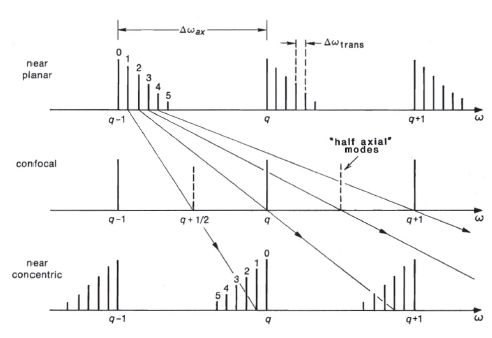
\includegraphics[clip,trim=0 0 0 2, width=0.9\linewidth]{Bild_2024-04-11_001906466}
	\caption{\blockquote{Resonance frequencies of higher order modes in
			optical resonators for different configurations.
		}\cite{gaussian_beam_script} Figure taken from \cite{gaussian_beam_script}}
	\label{fig:spektrum_cavities}
\end{figure}



